\chapter{Solution Design}
This chapter details and explains various aspects of the solution design. It begins with a explanation of the envisioned implementation of the solution in the clothing industry ecosystem. This is followed by a detailed account of the design process used to create the solution and lastly, an extensive overview of the experimental process used to test the solution.

\section{Implementation Design}

\subsection{Overview}
The solution aims to form part of larger practical implementation that will be applicable and provide relief in all three clothing channels mentioned in Section \ref{clothingIndustryContext}. However, in order to understand the needs the implementation must address, an analysis of pain points of consumers and producers in each channel must be performed. Shown in Table \ref{tab:conProdPainPoints} is a summary of such an analysis.

\begin{table}[htbp]
	\centering
	\caption{Pain points of consumers and producers in each of the three channels}
	\begin{tabularx}{\textwidth}{|Y|Y|Y|}
		\toprule
		& 
		\textit{\textbf{Consumers}} & 
		\textit{\textbf{Producers}} \\
		\midrule
		\textit{\textbf{Retail}} & 
		\begin{itemize}
			\item Visiting stores is time consuming
			\item Trying clothes on is tedious
			\item The correct size is often not available 
		\end{itemize} & 
		\begin{itemize}
			\item Dressing rooms waste valuable space
			\item Trying on clothes pose a security risk and require resources to control
			\item Significant costs are incurred during exchanges 
		\end{itemize} \\
		\midrule
		\textit{\textbf{Online}} & 
		\begin{itemize}
			\item Difficult to choose the correct size
			\item Not sure how the item will look on body
			\item Frustrating to exchange if item is incorrect
		\end{itemize} & 
		\begin{itemize}
			\item Exchanges severely impact their profitability
			\item Experience lower sale volume due as they cannot provide a complete customer experience
		\end{itemize}\\
		\midrule
		\textit{\textbf{Tailoring}} & 
		\begin{itemize}
			\item Only available for specialised clothing
			\item The process is time consuming
			\item There is always delay between getting measured and picking up clothing
		\end{itemize} & 
		\begin{itemize}
			\item Time required to complete measurements limits productivity
			\item Measurements can only take place in person with a trained tailor
		\end{itemize} \\
		\bottomrule
	\end{tabularx}%
	\label{tab:conProdPainPoints}%
\end{table}%


The aim of the overall implementation is to alleviate stresses on both consumers and suppliers that are inherent to the status quo.  In order to achieve this, the implementation will consist of the following key components: 

\begin{itemize}
	\item A compact, expedient and easy to use system that accurately measures the body parameters of a customer and provide clothing suggestions
	\item A platform that retains this customer information and creates a digital profile accessible to the customer and shareable between retailers  
	\item An intuitive interface that allows the customer to seamlessly get advise on clothing at his/her retailers of choice	
\end{itemize} 

A detailed end-to-end journey of the implementation is given in the following section.

\subsection{End-to-End Implementation Journey}

\begin{figure}[ht]
	\centering
	{%
		\setlength{\fboxsep}{0pt}%
		\setlength{\fboxrule}{0.5pt}%
		\fbox{
			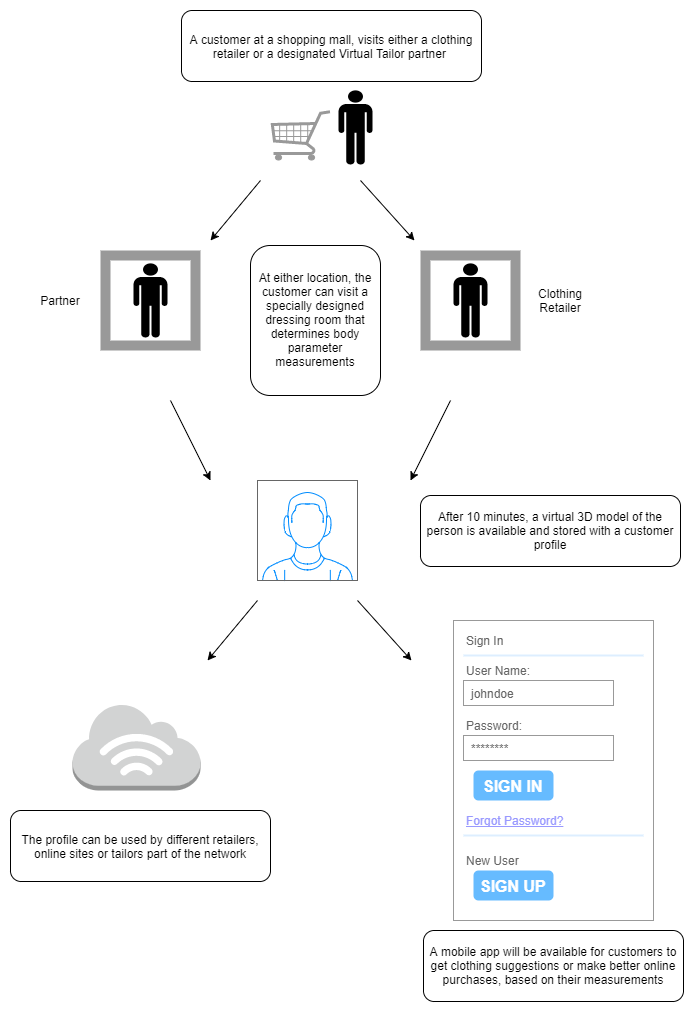
\includegraphics[width=0.8\textwidth]{End_to_End_Implementation.png}
	}}
	\caption{An illustration of the End-to-End journey of the envisioned implementation}
	\label{fig:endToEndImplementation}
\end{figure}


1) Online profile of people - Used for online shopping and retail shops\\
2) Take measurements at a retailer - Virtual Dressing room - A part of the shopping experience and will reduce hassle of trying on clothes\\
3) Amount wasted in trying on clothes or online returns?\\
4) Could be used for personalised tailoring
5) Example of UI - Explanation of how it works

\section{Component Selection}
1) Choice of Kinect - Compare to other depth sensors\\
- Kinect v1 vs v2
- Winddows vs Xbox
2) Choice of Windows SDK\\

\section{Algorithm Design}
1) Windows examples used - Background Removal, Colour Stream and Skeleton Tracking - NB - Why BackgroundRemoval instead of own method
3D Points - No calibration

2) Run through of algorithm
- Background Removed frame
- Send image to separate class for processing
- Create array with background removed pixels
- Draw skeleton on image
- Create axes for measurement - Perpendicular or straight depending on particular measurement

\section{Experimental Design}
- Constraints - Men, distance from Kinect, height of Kinect, Number of views, 3D Modelling, control distance - box of 0.5m
- UI to run simulated dressing room
- Volunteer to pose as instructed by person controlling UI
- Take measurement of front
- Take left
- Take back
- Take right 
- At each point, take actual readings with uncertainty
- Note: Did not use correction in \cite{nonContact2017}
- For one volunteer, take 5 readings in relatively the same pose - Determine uncertainty 